% INCLUDE A DEVISION OF LABOUR WHICH INDICATES THE CONTRIBUTIONS OF EACH MEMBER

\documentclass[12pt, titlepage]{article}

\usepackage{amssymb}
\usepackage{amstext}
\usepackage{amsthm}
\usepackage{amsmath}
\usepackage{enumerate}
\usepackage{fancyhdr}
\usepackage[margin=1in]{geometry}
\usepackage{graphicx}
\usepackage{extarrows}
\usepackage[shortlabels]{enumitem}
\usepackage{setspace}
\usepackage{tabu}
% Just a placeholder for now

\title{Group 11 SRS Document}

\author{}

\date{\today}

\begin{document}

\maketitle

\pagenumbering{roman}
\tableofcontents
\listoffigures

\newpage

\pagenumbering{arabic}

\section{Introduction}
This document provides the specifications for the software titled \textbf{Project Food} (this name is temporary and may change once a decision has been made among the development team). Henceforth, this project shall be referred to as Project Food for the entirety of this document.

This document is split into four major sections. The first (and current) section provides an introduction to the software. Section two elaborates on the overall description of the software. The third and fourth sections contain the functional and non-functional requirements of the product, respectively.

  \subsection{Purpose} 
  The purpose of this document is to present a functional description of Project Food. The document shall elaborate on the overall description, functional requirements, and non-functional requirements of the software. This document is intended for developers, stakeholders, and users of Project Food.
  \subsection{Scope}

  The primary product produced will be a desktop based application, namely Project Food. The purpose of the application is to provide entertainment to users by means of a 2D video game. Inspired by the popular game "The Binding of Isaac", users will indulge in a classic rogue-like video game experience by controlling a character, attacking enemies, and collecting items all while making decisions to visit unique procedurally-generated levels. In addition, users will have the ability to choose whether or not they wish to combine collected items, allowing them to upgrade features pertaining to their player. Upgrades will allow users to progress through the increasingly difficult levels, preparing them for various final boss fights.
  The application is intended to provide entertainment for all of its users. The application will be free to download from an application store, thereby maximizing the number of players using the application. The main goal of Project Food is to provide users a challenging, immersive, and friendly mobile video game form of entertainment with the classic rogue-like experience.
  \subsection{Definitions, Acronyms, and Abbreviations}
   
    \textbf{Agrovate}: To make an \textit{Enemy} aware of the \textit{Player's} presence. \\\\
    \textbf{Basic Attack}: The primary combat method of the \textit{Player}. \\\\
    \textbf{Basic Attack Key}: A user input that corresponds to the \textit{Player} performing a \textit{Basic Attack} in a cardinal direction (i.e. \textit{North Movement Key} corresponds to moving the \textit{Player} piece in the northern cardinal direction). \\\\
    \textbf{Boss}: A specialized \textit{Enemy} acting as the final challenge of a \textit{Map}. \\\\
    \textbf{Crafting}: The act of combining two or more items to create a new item.\\\\
    \textbf{Enemy}: Hostile game pieces that will attack the \textit{Player}. \\\\
    \textbf{Entities}: Objects that the player can interact with.\\\\
    \textbf{Ingredients}: The material items that are consumed during crafting.\\\\
    \textbf{Inventory}: The space that allows a player to store items, funds, and equipment.\\\\
    \textbf{Inventory Key}: A user input that corresponds to the opening the \textit{Player's} Inventory. \\\\
    \textbf{Levels}: A series of stages of incrementing difficulty that the player traverses.\\\\
    \textbf{Map}: A network of interconnected rooms that form the available playing space for the player.\\\\
    \textbf{Movement Key}: A user input that corresponds to moving the \textit{Player} in a cardinal direction (i.e. \textit{North Movement Key} corresponds to moving the \textit{Player} piece in the northern cardinal direction). \\\\
    \textbf{Player}: The central playing piece of the game and the avatar that the user controls to interact with the game.\\\\
    \textbf{Procedural Generation}: A method of creating data algorithmically as opposed to manually.\\\\
    \textbf{Rogue-like}: A subgenre of role-playing video game. \\\\
    \textbf{Skills}: Abilities that a player can acquire from playing the game that improve the combat effectiveness of the player.\\\\
    \textbf{Spawn Rooms}: The starting room that the player spawns in when entering a map for the first time.\\\\
    \textbf{Special Attack}: The secondary attack method of the player that has different effects based on the \textit{Player's} \textit{Skills}
    \textbf{Special Attack Key}: A user input that corresponds to the \textit{Player} using a \textit{Special Attack}. \\\\
    \textbf{Transition Area}: An area that loads the next \textit{Map} when the \textit{Player} enters it. \\\\
  
  \subsection{References}
  N/A
  \subsection{Overview}

  This document is organized into four major sections. Section one (the current section) provided an introduction of Project Food. The remaining three sections of this document are described in detail below. 

  The second section of this document contains the overall description of Project Food. This section will elaborate on the general factors that affect the product and its requirements. This will include the product perspective, the product functions, the user characteristics, constraints, and any relevant assumptions/dependencies.

  The third section of this document contains all of the software functional requirements pertaining to Project Food. These requirements provide the purpose for the products existence as they must meet the clients requirements.

  The fourth section of this document contains a list of the non-functional software requirements pertaining to Project Food. These requirements were created by the development team with the client in mind.

\section{Overall Description}

  \subsection{Product Perspective}
  This product is a 2-dimensional video game similar to many games on the market such as Binding of Isaac, Soul Knight, Pokémon, and more. Our video game fits in the adventure category for players. The product is independent and totally self-contained, it does not require any other extra programs or internet.
  
   \begin{figure}[htp]
        \centering
        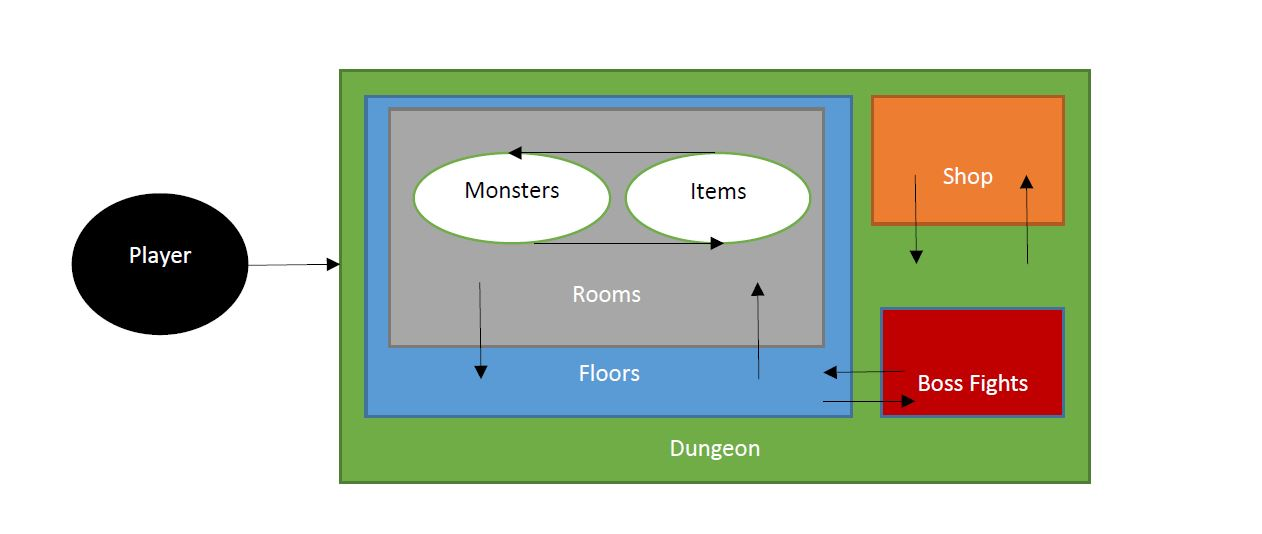
\includegraphics[width=16cm]{blckdg.JPG}
        \caption{Block Diagram}
        \label{fig:block}
   \end{figure}


  \subsection{Product Functions}
   \begin{center}
    \begin{tabular}{ | m{5em} | m{5em}| m{5em} | }
    \hline
    Player can start a new game & Player can enter a new room & Player can pick up an item \\
    \hline
    Player can craft an item & Player can enter a new level & Player can die \\
    \hline
    Player can start a transaction with the shop & Player can move the character & Player can fight other enemies \\
    \hline
    \end{tabular}
    \end{center}
  \subsection{User Characteristics}
  The education level required would be the completion of middle school. The user must have experience with playing platformer/dungeon crawling games and should know the overall objective of the game. Technical expertise is required for the use of the \textit{players} movement and action controls and volume adjustment.
  \subsection{Constraints}
  Time will limit the development of the game as we only have a couple of months before its completion. University course load, midterms, and labs will also be a limiting factor. The user is constrained by the interface of the game and the four directional movements of the player. A mouse and keyboard is also a constraint for game, because it is crucial that there is a mouse and keyboard for the game to function. 
  \subsection{Assumptions and Dependencies}
  One assumption about the game is that it will be played on computers that have enough performance capacity. If the computer does not have enough hardware resources available for the application, there may be scenarios where the application does not work as intended or even at all. Another assumption is that the mouse and keyboard of all computers work in the same way. If the keyboards have different functions for the arrow keys for example, the player may not be able to move.
  \subsection{Apportioning of Requirements}
  In the case that the project is delayed, there are some requirements that could be transferred to the next version of the game. Those requirements are to be developed in the second version.

\section{Functional Requirements}

\begin{enumerate}[{VP}1.]
  \item User 

  \begin{enumerate}[{BE1}.1]

    \item The user wants to start game.
    \begin{enumerate}
      \item The system presents a menu with the option of starting a new game or loading a previous save file.
      \item The user must be able to select either option of starting a new game or loading a previous save.
      \item If load game is selected, a list of all save files is presented.
      \item Each save file must be selectable.
    \end{enumerate}

    \item The user starts a new game.
    \begin{enumerate}
      \item A \textit{Level 1 Map} must be generated.
      \item The \textit{Player} must be placed in the \textit{Spawn Room}.
      \item The \textit{Player's} \textit{Inventory} must be created.
    \end{enumerate}

    \item The user loads a game.
    \begin{enumerate}
      \item The map must be loaded from the save file.
      \item The \textit{Player} must be placed in the \textit{Spawn Room}.
      \item The \textit{Player's Inventory} must be loaded from the save file.
      \item All previously attained \textit{Skills} must be loaded from the save file.
    \end{enumerate}

    \item The user wants to traverse the map.
    \begin{enumerate}
      \item The \textit{Player} must move in the direction given by the user's input.
      \item Each room must have at least one passage to another room or level.
      \item The \textit{Player} must be able to enter through each passage.
      \item Each room must have associated \textit{entities}.
      \item The state of each room must be saved when exited.
      \item A newly entered room must generate all of its \textit{entities}.
      \item A previously entered room must reload its most recently saved state.
    \end{enumerate}

    \item The user wants to buy an item.
    \begin{enumerate}
      \item Each \textit{Map} generated must have at least one \textit{Shop}.
      \item Each \textit{Shop} must have a list of items with an associated cost.
      \item The \textit{Player} must be able to interact with the shop.
      \item The \textit{Player} must be able to purchase items from the \textit{Shop} if they have sufficient funds in their \textit{Inventory}.
    \end{enumerate}

    \item The user wants to craft an item.
    \begin{enumerate}
      \item The user must be able to open a menu listing all of the \textit{Player} owned items.
      \item The \textit{Player} must be able to combining two or more items in their \textit{Inventory} to create new items.
      \item If an item is \textit{Crafted}, it is added to the \textit{Inventory} and its \textit{Ingredients} are removed from the \textit{Inventory}.
    \end{enumerate}

    \item The user wants to move the \textit{Player}.
    \begin{enumerate}
      \item The user inputs a \textit{Movement Key} without prompt from the system.
      \item The \textit{Player} responds by moving in the direction of the inputed \textit{Movement Key} (i.e. \textit{North Movement Key} corresponds to moving the \textit{Player} piece in the northern cardinal direction).
      \item The \textit{Player} will not be able to move through collidable \textit{Entities}.
    \end{enumerate}

    \item The user wants to perform a \textit{Basic Attack}.
    \begin{enumerate}
      \item The user inputs a \textit{Basic Attack Key} without prompt from the system.
      \item The \textit{Player} responds by performing a \textit{Basic Attack} in the direction of the inputed \textit{Movement Key} (i.e. \textit{North Movement Key} corresponds to moving the \textit{Player} piece in the northern cardinal direction).
      \item \textit{Basic Attacks} that hit collidable \textit{Entities} that are not \textit{Enemies} will be destroyed on those \textit{Entities}.
    \end{enumerate}

    \item The user wants to perform a \textit{Special Attack}.
    \begin{enumerate}
      \item The user inputs the \textit{Special Attack Key} without prompt from the system.
      \item The \textit{Player} responds by performing a \textit{Special Attack} in the cardinal direction the \textit{Player} is facing.
      \item \textit{Special Attacks} that hit collidable \textit{Entities} that are not \textit{Enemies} will be destroyed on those \textit{Entities}.
    \end{enumerate}
    
    \item The user wants to open the \textit{Player's Inventory}.
    \begin{enumerate}
      \item The user inputs the \textit{Inventory Key} without prompt from the system.
      \item The \textit{Player's} inventory screen is rendered for the user.
      \item The user can press the \textit{Inventory Key} again to close the \textit{Player's} inventory screen.
    \end{enumerate}

    \item The user initiates combat with an \textit{Enemy}.
    \begin{enumerate}
      \item The \textit{Player} \textit{Agrovates} an \textit{Enemy} by attacking it.
      \item \textit{Basic Attacks} that hit an \textit{Enemy} will apply damage to that \textit{Enemy}.
      \item \textit{Special Attacks} that hit an \textit{Enemy} will apply damage and other effects defined by the attack.
      \item If the \textit{Player} is hit by an \textit{Enemy} attack, the \textit{Player} will take damage.
      \item If an \textit{Enemy} dies, it will drop an \textit{Ingredient}.
    \end{enumerate}

    \item The user initiates combat with a \textit{Boss}.
    \begin{enumerate}
      \item The \textit{Player} \textit{Agrovates} a \textit{Boss} by attacking it.
      \item \textit{Basic Attacks} that hit a \textit{Boss} will apply damage to those \textit{Enemies}.
      \item \textit{Special Attacks} that hit \textit{Enemies} will apply damage and other effects defined by the attack.
      \item If the \textit{Player} is hit by a \textit{Boss's} attack, the \textit{Player} will take damage.
      \item If the \textit{Boss} is defeated, the \textit{Player} will be allowed to transition to the next \textit{Map}.
    \end{enumerate}

    \item The user enters a \textit{Map Transition}.
    \begin{enumerate}
      \item The user must have defeated the \textit{Boss} in the current \textit{Map}.
      \item The \textit{Player} must enter a corresponding transition area to the \textit{Map}.
      \item The next \textit{Map} will be gernerated and the \textit{Player} will be placed in its \textit{Spwan Room}.
    \end{enumerate}

  \end{enumerate}
\end{enumerate}

\section{Non-Functional Requirements}
\label{sec:non-functional_requirements}
% Begin Section
\subsection{Look and Feel Requirements}
\label{sub:look_and_feel_requirements}
% Begin SubSection

\subsubsection{Appearance Requirements}
\label{ssub:appearance_requirements}
% Begin SubSubSection
\begin{enumerate}[{LF}1. ]
        \item The game interface shall be easy and clear for users to operate.
        \item The game must not contain any frightening scenes.
\end{enumerate}
% End SubSubSection

\subsubsection{Style Requirements}
\label{ssub:style_requirements}
% Begin SubSubSection
\begin{enumerate}[{LF}3. ]
        \item The user should feel that the gameplay increases in difficulty as their game progress increases
\end{enumerate}
% End SubSubSection

% End SubSection

\subsection{Usability and Humanity Requirements}
\label{sub:usability_and_humanity_requirements}
% Begin SubSection

\subsubsection{Ease of Use Requirements}
\label{ssub:ease_of_use_requirements}
% Begin SubSubSection
\begin{enumerate}[start=1,label={ UH\arabic*.}]
        \item Gameplay shall be easy for a person of 10 years of age or older to learn.
\end{enumerate}
% End SubSubSection

\subsubsection{Personalization and Internationalization Requirements}
\label{ssub:personalization_and_internationalization_requirements}
% Begin SubSubSection
N/A
% End SubSubSection

\subsubsection{Learning Requirements}
\label{ssub:learning_requirements}
% Begin SubSubSection
\begin{enumerate}[start=2,label={ UH\arabic*.}]
        \item It shall take a maximum time of 5 minutes to learn the basic operation
        \item After a full read through of the provided instruction manual, the user should be able to use all in-game functionality with ease
\end{enumerate}
% End SubSubSection

\subsubsection{Understandability and Politeness Requirements}
\label{ssub:understandability_and_politeness_requirements}
% Begin SubSubSection
\begin{enumerate}[start=4,label={ UH\arabic*.}]
        \item All in game icons shall be taken from their common usage icons where applicable.
        \item The appearance of all food enemies will be intuitive to their physical appearance
        \item New terminology used in game shall come with a brief explanation of their meaning
        \item Ambiguous language, such as words with conflicting alternate meanings, used in in-game decisions shall have their meaning clarified

\end{enumerate}
% End SubSubSection

\subsubsection{Accessibility Requirements}
\label{ssub:accessibility_requirements}
% Begin SubSubSection
\begin{enumerate}[start=8,label={ UH\arabic*.}]
        \item The game navigation shall be based on the standard PC control scheme of using WASD mapping, and the mouse.
        \item All in game elements will have high contrast with surrounding elements to aid colour blind users
        \item All fonts used for in-game text shall be deemed accessible
        \item All information communicated via sound shall have an accompanying box of text transcribing the information
        \item The user should be able to mute or reduce the volume of in-game sound effects and music
        \item The user should be provided with an epilepsy warning in advance of scenes with flashing lights or rapidly changing colours

\end{enumerate}
% End SubSubSection

% End SubSection

\subsection{Performance Requirements}
\label{sub:performance_requirements}
% Begin SubSection

\subsubsection{Speed and Latency Requirements}
\label{ssub:speed_and_latency_requirements}
% Begin SubSubSection
\begin{enumerate}[{PR}1. ]
        \item The response time shall be within 1 ms.
        \item Setting up a new game shall take no more than 5 seconds.
\end{enumerate}
% End SubSubSection

\subsubsection{Safety-Critical Requirements}
\label{ssub:safety_critical_requirements}
% Begin SubSubSection
N/A
% End SubSubSection

\subsubsection{Precision or Accuracy Requirements}
\label{ssub:precision_or_accuracy_requirements}
% Begin SubSubSection
N/A
% End SubSubSection

\subsubsection{Reliability and Availability Requirements}
\label{ssub:reliability_and_availability_requirements}
% Begin SubSubSection
\begin{enumerate}[start=3,label={ PR\arabic*.}]
        \item The game shall be able to run 24 hours per day, 365 days per year.
\end{enumerate}
% End SubSubSection

\subsubsection{Robustness or Fault-Tolerance Requirements}
\label{ssub:robustness_or_fault_tolerance_requirements}
% Begin SubSubSection
\begin{enumerate}[start=4,label={ PR\arabic*.}]
        \item The game shall not be affected, such as information loss, due to any internet issue.
\end{enumerate}
% End SubSubSection

\subsubsection{Capacity Requirements}
\label{ssub:capacity_requirements}
% Begin SubSubSection
\begin{enumerate}[start=5,label={ PR\arabic*.}]
        \item The game shall store achievement data for up to one player

\end{enumerate}
% End SubSubSection

\subsubsection{Scalability or Extensibility Requirements}
\label{ssub:scalability_or_extensibility_requirements}
% Begin SubSubSection
N/A
% End SubSubSection

\subsubsection{Longevity Requirements}
\label{ssub:longevity_requirements}
% Begin SubSubSection
N/A
% End SubSubSection

% End SubSection

\subsection{Operational and Environmental Requirements}
\label{sub:operational_and_environmental_requirements}
% Begin SubSection

\subsubsection{Expected Physical Environment}
\label{ssub:expected_physical_environment}
% Begin SubSubSection
N/A
% End SubSubSection

\subsubsection{Requirements for Interfacing with Adjacent Systems}
\label{ssub:requirements_for_interfacing_with_adjacent_systems}
% Begin SubSubSection
N/A
% End SubSubSection

\subsubsection{Productization Requirements}
\label{ssub:productization_requirements}
% Begin SubSubSection
N/A
% End SubSubSection

\subsubsection{Release Requirements}
\label{ssub:release_requirements}
% Begin SubSubSection
\begin{enumerate}[{OE}1. ]
        \item Maintenance releases that fix an error within the game shall be available as soon as they are produced
        \item Feature releases will be comprised of numerous features and will be released with a maximum monthly frequency
\end{enumerate}
% End SubSubSection

% End SubSection

\subsection{Maintainability and Support Requirements}
\label{sub:maintainability_and_support_requirements}
% Begin SubSection

\subsubsection{Maintenance Requirements}
\label{ssub:maintenance_requirements}
% Begin SubSubSection
\begin{enumerate}[{MS}1. ]
        \item Levels should be modifiable after the product's release
        \item Floors should be modifiable after the product's release
        \item The ability to add new levels (and floors) after the product's release should be available
        \item The variety of food should be modifiable after the product's release.
\end{enumerate}
% End SubSubSection

\subsubsection{Supportability Requirements}
\label{ssub:supportability_requirements}
% Begin SubSubSection
\begin{enumerate}[start=5,label={ MS\arabic*.}]
        \item The game shall provide the user with a comprehensive set of instructions
        \item The game shall provide the user with a set of Frequently Asked Questions
        \item The game shall provide the user with a detailed explanation of the functionality of each item that may appear.
\end{enumerate}
% End SubSubSection

\subsubsection{Adaptability Requirements}
\label{ssub:adaptability_requirements}
% Begin SubSubSection
\begin{enumerate}[start=8,label={ MS\arabic*.} ]
        \item The game is expected to run under Windows and Linux operating system
\end{enumerate}
% End SubSubSection

% End SubSection

\subsection{Security Requirements}
\label{sub:security_requirements}
% Begin SubSection

\subsubsection{Access Requirements}
\label{ssub:access_requirements}
% Begin SubSubSection
N/A
% End SubSubSection

\subsubsection{Integrity Requirements}
\label{ssub:integrity_requirements}
% Begin SubSubSection
N/A
% End SubSubSection

\subsubsection{Privacy Requirements}
\label{ssub:privacy_requirements}
% Begin SubSubSection
N/A
% End SubSubSection

\subsubsection{Audit Requirements}
\label{ssub:audit_requirements}
% Begin SubSubSection
N/A
% End SubSubSection

\subsubsection{Immunity Requirements}
\label{ssub:immunity_requirements}
% Begin SubSubSection
N/A
% End SubSubSection

% End SubSection

\subsection{Cultural and Political Requirements}
\label{sub:cultural_and_political_requirements}
% Begin SubSection

\subsubsection{Cultural Requirements}
\label{ssub:cultural_requirements}
% Begin SubSubSection
\begin{enumerate}[{CP}1. ]
        \item The game shall not include any features that could be considered offensive in any of our market countries.
\end{enumerate}
% End SubSubSection

\subsubsection{Political Requirements}
\label{ssub:political_requirements}
% Begin SubSubSection
\begin{enumerate}[]
        \item N/A
\end{enumerate}
% End SubSubSection

% End SubSection

\subsection{Legal Requirements}
\label{sub:legal_requirements}
% Begin SubSection

\subsubsection{Compliance Requirements}
\label{ssub:compliance_requirements}
% Begin SubSubSection
\begin{enumerate}[{LR}1. ]
        \item All game asset shall be compliant with the Web Content Accessibility Guidelines
\end{enumerate}
% End SubSubSection

\subsubsection{Standards Requirements}
\label{ssub:standards_requirements}
% Begin SubSubSection
N/A
% End SubSubSection

% End SubSection

% End Section

\newpage

\section{Division of Labour}

Andrew Lucentini  - Section 1: \\\\\\
Rafen Hussain     - Section 2: \\\\\\
Alex Lo           - Section 3 (be1-be6 inclusive): \\\\\\
Lucas Zacharewicz - Section 3 (be7-be13 inclusive): \\\\\\
Chen Shuying      - Section 4 (in collaboration with Alexie McDonald): \\\\\\
Alexie McDonald   - Section 4 (in collaboration with Chen Shuying): \\\\\\
\end{document}

